\documentclass[german,  % Standardmäßig deutsche Eigenarten, englisch -> english
parskip=full,  % Absätze durch Leerzeile trennen
%bibliography=totoc,  % Literatur im Inhaltsverzeichnis (ist unüblich)
%draft,  % TODO: Entwurfsmodus -> entfernen für endgültige Version
headsepline]{scrartcl}
\usepackage[utf8]{inputenc}  % Kodierung der Datei
\usepackage[T1]{fontenc}  % Vollen Umfang der Schriftzeichen
\usepackage[german]{babel}  % Sprache auf Deutsch (neue Rechtschreibung)
\usepackage{booktabs}
\usepackage{float}
% Mathematik und Größen
\usepackage{amsmath}
\usepackage[locale=DE,  % englische Eigenarten, deutsch -> DE
separate-uncertainty,  % Unsicherheiten seperat angeben (mit ±)
]{siunitx}
%http://texdoc.net/texmf-dist/doc/latex/siunitx/siunitx.pdf
\usepackage{physics}  % Erstellung von Gleichungen vereinfachen
\usepackage{svg}    
\usepackage{graphicx}  % Bilder einbinden \includegraphics{Pfad/zur/Datei(ohne Dateiendung)}
\usepackage{biblatex}
\usepackage[version=4,arrows=pgf]{mhchem}  % Chemie Paket für Isotopenschreibweise etc.
\usepackage{wrapfig}
\usepackage{floatflt}
\usepackage{enumerate}
% Gestaltung
%\usepackage{microtype}  % Mikrotypographie (kann man am Ende verwenden)
\usepackage{booktabs}  % schönere Tabellen
%\usepackage[toc]{multitoc}  % mehrspaltiges Inhaltsverzeichnis
\usepackage{multicol}
\usepackage{csquotes}  % Anführungszeichen mit \enquote
\usepackage{caption}  % Anpassung der Bildunterschriften, Tabellenüberschriften
\usepackage{subcaption}  % Unterabbildungen, Untertabellen, …
\usepackage{cprotect}
\usepackage{enumitem}  % Listen anpassen
\usepackage{siunitx}
\usepackage{eufrak}
\usepackage{dirtytalk}
\usepackage{subcaption}
\usepackage{textcomp}
\setlist{itemsep=-10pt}  % Abstände zwischen Listenpunkten verringern

% Manipulation des Seitenstils
\usepackage{scrlayer-scrpage}
% Kopf-/Fußzeilen setzen
\pagestyle{scrheadings}  % Stil für die Seite setzen
\clearscrheadings  % Stil zurücksetzen, um ihn neu zu definieren
\automark{section}  % Abschnittsnamen als Seitenbeschriftung verwenden
\ofoot{\pagemark}  % Seitenzahl außen in Fußzeile
\ihead{\headmark}  % Seitenbeschriftung mittig in Kopfzeile
%\setkomafont{\headsepline}{}
\setcounter{tocdepth}{2} %set depth of printed table of contets.

\makeatletter

%\renewcommand\tableofcontents{% Absatz vor Gliederungspunkten
   % \begin{multicols}{2}[\section*{\contentsname
 %       \@mkboth{%
  %         \MakeUppercase\contentsname}{\MakeUppercase\contentsname}}]%
 %   \@starttoc{toc}%
 %   \end{multicols}%
 %   }

\makeatother %print dots in sections in toc.

\usepackage[hidelinks]{hyperref}  % Links und weitere PDF-Features
\usepackage[]{cleveref} %noabbrev für ausgeschriebene verweise
% TODO: Titel und Autor, … festlegen
\newcommand*{\titel}{Mössbauerspektroskopie}
\newcommand*{\autor}{Steven Gebel, Lukas König}
\newcommand*{\abk}{}
\newcommand*{\betreuer}{Felix Seewald}
\newcommand*{\messung}{22. Oktober 2021}
\newcommand*{\ort}{REC/D011}
\newcommand{\diff}[1]{\frac{\mathrm{d}}{\mathrm{d}#1}}
\newcommand{\mum}{\:\si{\mu m\:}}
\newcommand{\ten}[1]{\cdot10^{#1}}
\newcommand{\dsys}{\Delta_\text{sys}}
\newcommand{\logdiff}[1]{\left(\frac{\Delta #1}{#1}\right)^2}
\newcommand{\dunderline}[1]{\underline{\underline{#1}}}
\newcommand{\bcref}[1]{\namecref{#1} \textcolor{blue}{\labelcref{#1}}}

\hypersetup{pdfauthor={\autor}, pdftitle={\titel}}  % PDF-Metadaten setzen

% automatischen Titel konfigurieren
\titlehead{Fortgeschrittenenpraktikum MBS\abk \hfill Technische Universität Dresden}
\subject{Praktikumsbericht}
\title{\titel}
\author{\autor}
\date{\begin{tabular}{ll}
Protokoll: & \today\\
Messung: & \messung\\
Versuchsplatz: & \ort\\
Betreuer: & \betreuer\end{tabular}}
\begin{document}
\begin{titlepage}
\maketitle  % Titel setzen
\tableofcontents  % Inhaltsverzeichnis setzen
\end{titlepage}
\section{Einleitung}
\subsection{Aufgabenstellung}
\begin{itemize}
    \item Aufnahme des Pulshöhenspektrums der Quelle, Identifizierung der Mößbauerlinie und
anderer Linien, Kalibrierung der x-Achse des Pulshöhenspektrums, setzen des Gamma-
fensters für die 14.4 keV-Linie
\item Kalibrierung des Mößbauerantriebs mit Hilfe einer Eisenfolie
\item Bestimmung der Hyperfeinparameter von Ferrocen
\item Bestimmung des Materials einer unbekannten Probe
\end{itemize}

\subsection{Theoretischer Hintergrund}
Die \textsc{Mößbauerspektroskopie} ist eine wichtige Methode um über die Untersuchung von Hyperfeinwechselwirkungen kernphysikalische und festkörperphysikalische Informationen zu gewinnen.\\
Der Erfolg und die große Relevanz dieser Methode ist mit ihrer hohen Auflösungsmöglichkeit und der Tatsache begründet, dass mit ihr etwa 45 Elemente untersucht werden können, wobei das Isotop $^{57}$Fe mit seiner hohen physikalischen und technischen Bedeutung darunter fällt. Ihr Entdecker Rudolf Mößbauer erhielt für seine Forschungen mit diesem Effekt 1961 den Nobelpreis.

\subsubsection{Mößbauer-Effekt}
Der namensgebende Effekt der Mößbauerspektroskopie ist ein Resonanzabsorptionsexperiment. Genauer handelt es sich um rückstoßfreie Kernresonanzabsorption von Gammastrahlung.\\
Ein Photon mit Impuls $\hbar \Vec{k}_{\gamma}$ kann diesen auf einen Atomkern übertragen und somit anregen. Damit ist ein Energieverlust 
\begin{equation}
    \Delta E_{\gamma} = \frac{-E_{\gamma}^2}{2Mc^2} \approx \frac{-E_{0}^2}{2Mc^2} 
\end{equation}
verbunden. Dieser soll möglichst klein werden um Resonanz zwischen emittierenden Kernen und absorbierenden Kernen zu erreichen, was offensichtlich dann erreichbar ist, wenn entweder $E_0$ (Energiedifferenz der Elektronenniveaus) klein ist, oder der Rückstoß auf ein ganzes Atomgitter übertragen wird und somit $M$ sehr groß wird, was sich in der Mößbauerspektroskopie zu Nutze gemacht wird.\\
$^{57}$Fe ist der bedeutendste Mößbauerspektroskopie-Kern, wobei das Zerfallsschema in \bcref{fig:aufbau} dargestellt ist.\\
Das Messprinzip beruht auf einer periodisch bewegten Quelle einer radioaktiven Substanz. Durch die Geschwindigkeitsvariation werden durch den linearen Dopplereffekt die $14.4$ keV-$\gamma$-Quanten des $^{57}$Fe leicht in ihrer Energie variiert. Im Absorberkern treten Hyperfeinwechselwirkungen auf, weswegen die Energieaufspaltungen im Bereich von $\approx 100\, \si{neV}$ nicht direkt durch einen Gammadetektor erfasst werden können, sondern stattdessen die in einem bestimmten Gammafenster liegenden Photonen mit der Dopplergeschwindigkeit $v$ assoziiert werden und letztlich das Absorptionsspektrum $I = I(v\text{(channel)})$ als Mößbauerspektrum interpretiert wird.

\begin{figure}[h!]
    \centering
    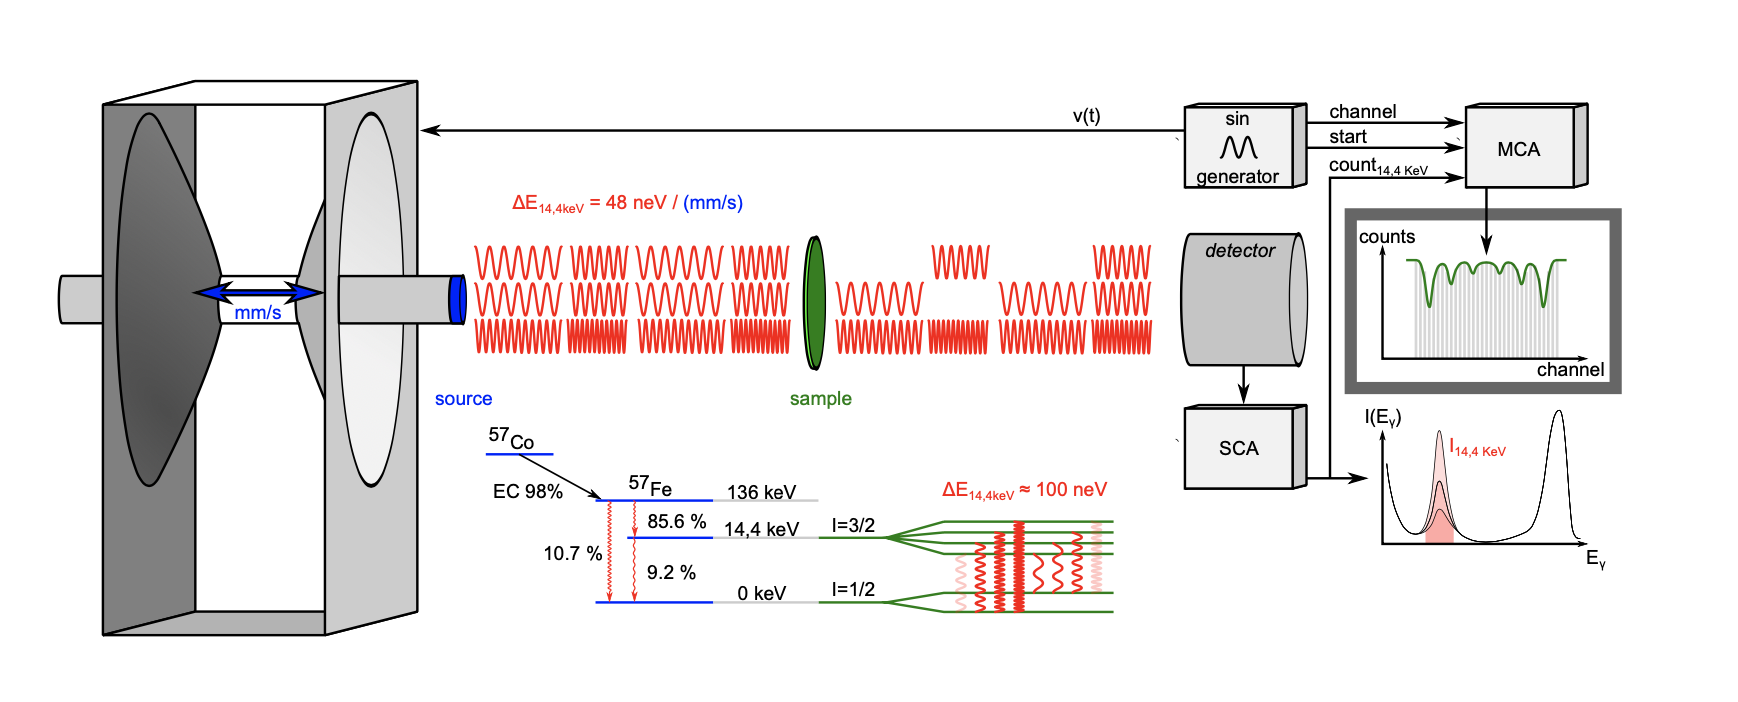
\includegraphics[width=1.05\linewidth]{mbs_aufbau.png}
    \caption{Energieniveauschema von $^{57}$Fe, bzw. Kern-Zeeman-Aufspaltung und allgemeines Messprinzip der Mößbauerspektroskopie in Transmissionsgeometrie.}
    \label{fig:aufbau}
\end{figure}
\subsubsection{Hyperfeinwechselwirkung}
Die Hyperfeinwechselwirkungen des Sondenkerns mit seiner elektronischen Umgebung heben die Energieentartung der Kernzustände $\ket{I,I_z}$ auf. Im Folgenden werden die verschiedenen auftretenden Wechselwirkungen näher beschrieben.
\begin{figure}[htp!]
    \centering
    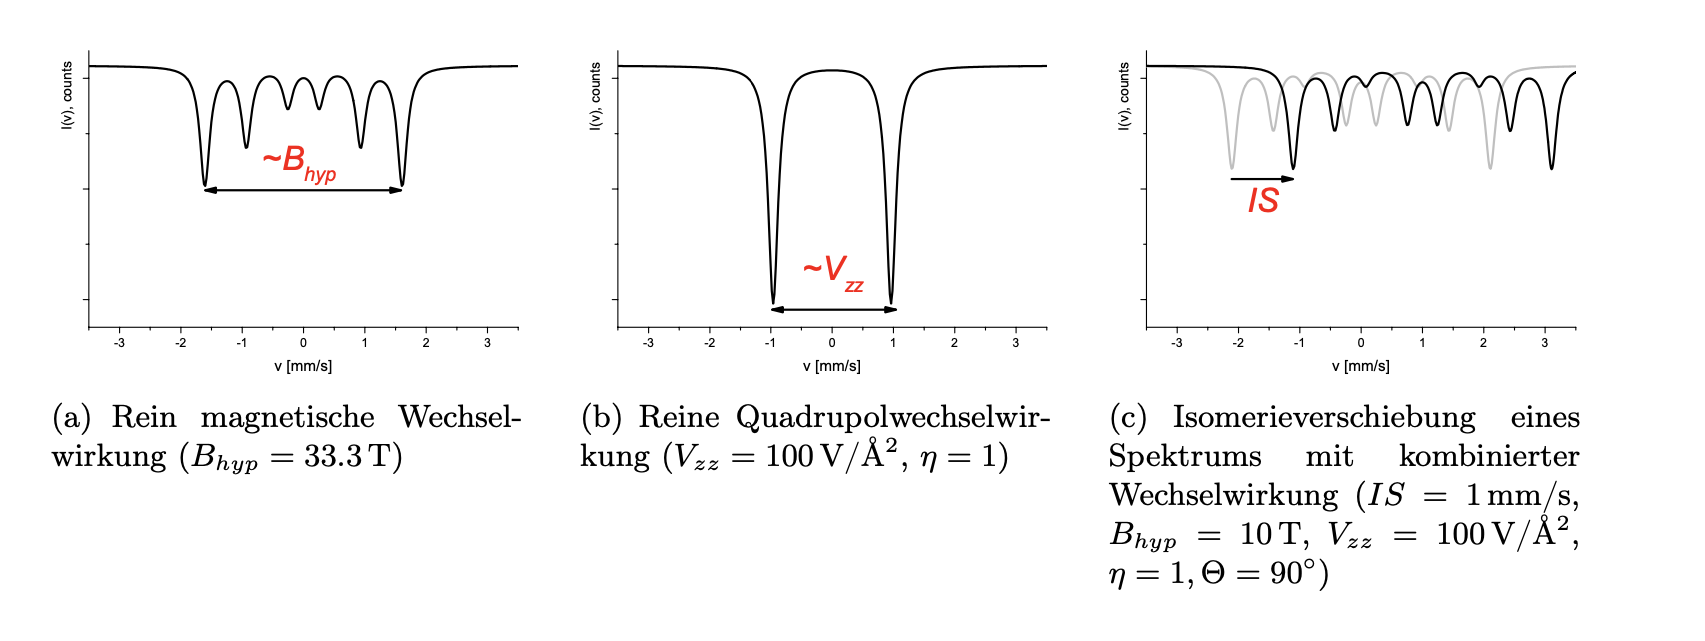
\includegraphics[width=1.05\linewidth]{mbs_ww.png}
    \caption{Bedeutung der Hyperfeinwechselwirkungen im $^{57}$Fe-Mößbauerspektrum.}
    \label{fig:ww}
\end{figure}
\begin{figure}[htp!]
    \centering
    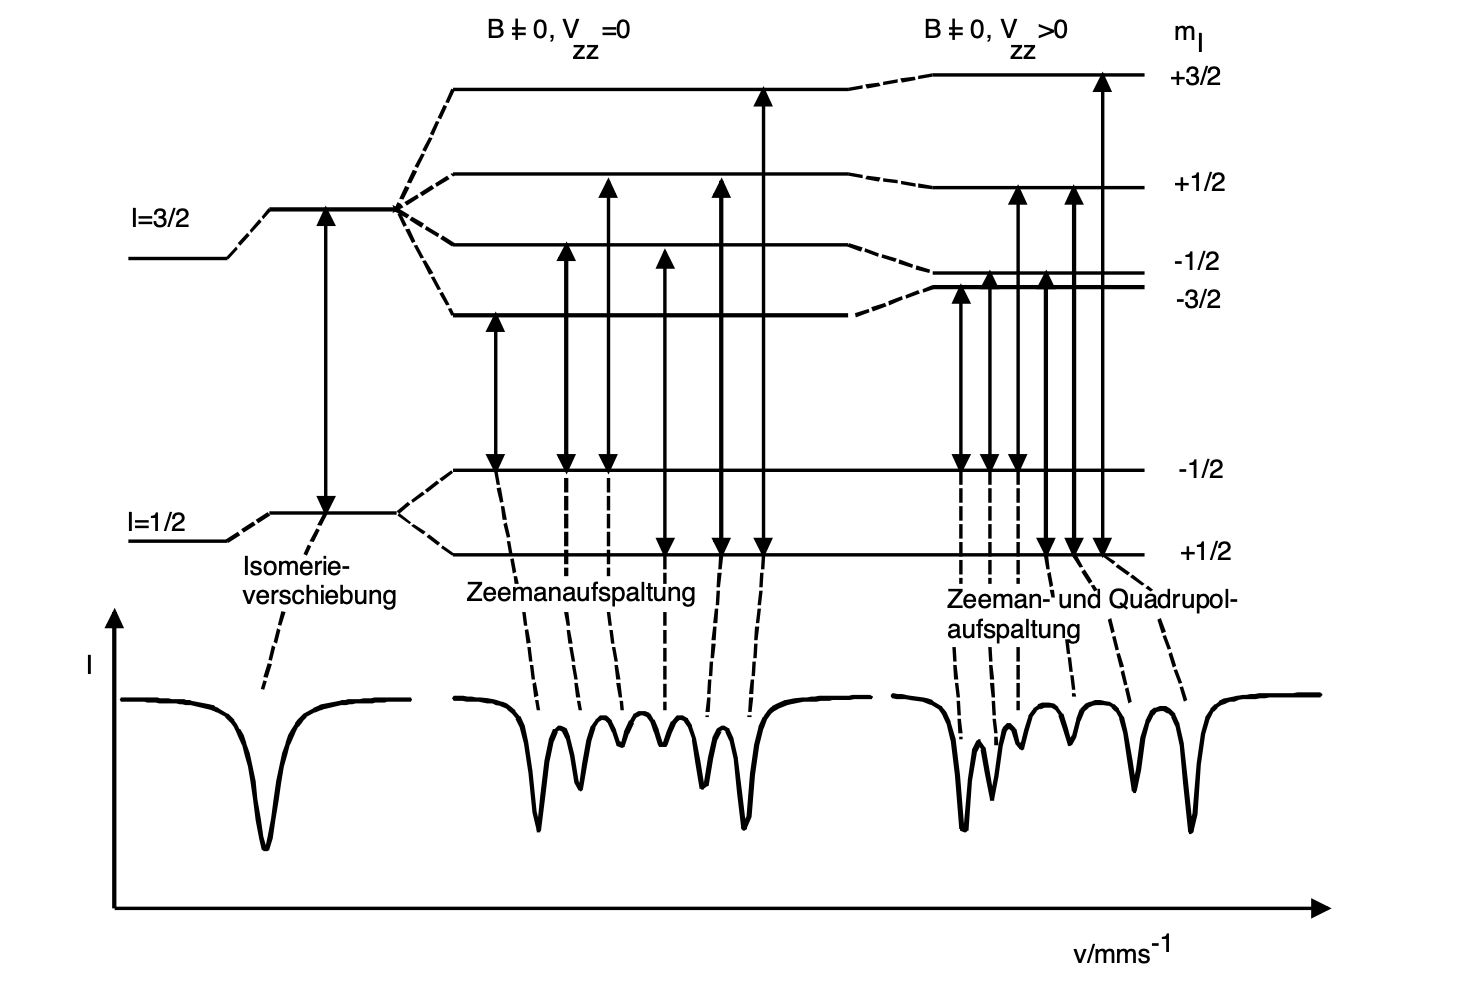
\includegraphics[width=0.65\linewidth]{mbs_aufspaltung.png}
    \caption{Magnetische Aufspaltung durch verschiedene Hyperfeinwechselwirkungen und resultierende  Mößbauer-Spektren  (schematisch). Die Isomerieverschiebung ergibt sich aus der Lage des Signalschwerpunkts. (\href{https://www.uni-muenster.de/imperia/md/content/physikalische_chemie/app_moess.pdf}{\textcolor{blue}{Quelle}, Stand: 29.10.2021})}
    \label{fig:aufspaltung}
\end{figure}


\paragraph{Zeemanaufspaltung}
Der Kern-Zeemaneffekt, verursacht durch den Kernspin $\Vec{\mu}=g_I\mu_n\frac{\Vec{I}}{\hbar}$ im magnetischen Feld $\Vec{B}$ erzeugt durch den Gesamtdrehimpuls $\Vec{I}$ der Hüllenelektronen, wobei weiterhin für die s-Elektronen mit Aufenthaltswahrscheinlichkeit im Kern die Fermi-Kontakt-Wechselwirkung hinzugezogen werden muss, wird vereinfacht durch folgenden Hamiltonoperator beschrieben:
\begin{equation}
    \mathcal{H}_Z = -\Vec{\mu}\Vec{B}=-g_I\mu_nI_zB_z
\end{equation}
\label{zeeman}
Es gibt also $2I+1$ energetisch äquidistante Unterzustände in den Kernniveaus, wobei beim betrachteten $^{57}$Fe die Kernspinquantenzahlen $I=1/2$ und $I=3/2$ zu beachten sind.\\
Unter Berücksichtigung der Tatsache, dass Übergänge mit $\Delta I_z=\pm2$ verboten sind, ist bei reiner Zeemanaufspaltung ein charakteristisches Sextett zu erwarten.\\
Die Verhältnisse der Linienintensitäten unter reiner Zeemanaufspaltung verhalten sich, wie 3:2:1:1:2:3.

\paragraph{Quadrupolaufspaltung und Isomerieverschiebung}
\label{quad}
Quadrupolaufspaltung und Isomeriverschiebung resultieren aus der Kernladungsdichte $\rho(\Vec{r})$ und dem elektrischen Potential $\Phi(\Vec{r})$ seiner Umgebung. Wenn das durch das Potential erzeugt elektrische Feld nur schwach im von der Verteilung $\rho$ besetzen Bereich variiert, kann die Energie der Kernladung $\mathcal{H}_{el}=\int d^3r\rho(\Vec{r})\Phi(\Vec{r})$ in einer Taylorreihe bis zur zweiten Ordnung entwickelt werden um den Ursprung von $\Vec{r}$, womit sich nach Transformation in das Hauptachsensystem des elektrischen Potentials ergibt: 
\begin{equation}
    \mathcal{H}_{el} \approx Ze\Phi(0) - \frac{Ze<r^2>\rho_e(0)}{6\epsilon_0} + \frac{e}{6}\sum_i^3 V_{ii}Q_{ii}
\end{equation}
Der erste Term ist die elektrostatische Energie des als punktförmig angenommenen Kerns und im Weiteren uninteressant.\\ Der zweite Term spiegelt die Isomerieverschiebung wieder, wobei die Poissongleichung $\Delta \Phi(0)=-\frac{\rho_e(0)}{\epsilon_0}$ für die Ladungsdichte des Kerns verwendet wurde. Es tragen also nur s-Elektronen und der mittlere quadratische Kernradius $<r^2>$, welcher abhängig von der Hauptquantenzahl $I$ ist, zur Isomerieverschiebung bei. Somit ist das Ergebnis eine äquidistante Verschiebung aller Übergangsenergien.\\ Der dritte Term beschreibt die Quadrupolwechselwirkung, wobei das Kernquadrupolmoment $Q_{ii}$ mit dem elektrischen Feldgradienten $V_{ii} = \Phi_{ii}-\frac{\Delta \Phi}{3}$ wechselwirkt. Nun kann man mithilfe des Wigner-Eckhart-Theorems und unter Einführung des  Asymmetrieparameter $\eta:= \frac{V_{xx}-V_{yy}}{V_{zz}}$ und Auf- bzw. Absteigeoperatoren $I_+$, $I_-$ schreiben:
\begin{equation}
    \mathcal{H}_{el} = \frac{eQ_{zz}V_{zz}}{4I(2I-1)}\left [ (3I_z^2-I^2)+\frac{\eta}{2}(I_+^2+I_-^2)\right]
\end{equation}
Wichtig ist hier, dass die Quadrupolwechwirkungsenergie den Operator $I_z$ nur quadriert enthält, was bedeutet, dass Kernzustände $\ket{I,I_z}$, mit bis auf das Vorzeichen gleichem $I_z$, zweifach entartet bleiben. Da nur Kerne mit $I>1/2$ ein nicht verschwindendes Quadrupolmoment haben ist zu erwarten, dass nur für $I=3/2$ des $^{57}$Fe-Kerns zwei jeweils zweifach entartete Unterzustände auftreten, die dann im Mößbauerspektrum als charakteristisches Dublett zu sehen sind.\footnote{Vgl. Barb, D., 1980, Grundlagen und Anwendungen der Mössbauerspektroskopie, S.109 ff.}\\
Das Verhältnis der Linienintensitäten des Dubletts ist 1:1.

\subsubsection{Ferrocen}
Der in diesem Versuch verwendete Komplex Ferrocen ist in seiner Struktur bestehend aus einem zentralen Eisenkation der Oxidationsstufe II, welches eingelagert zwischen zwei Cyclopentadienylanionen ($\ce{C5H5-}$) liegt, die parallel zueinander im gleichen Abstand zum Eisen(II)-Kation liegen.
Der Abstand der Kohlenwasserstoffgruppen beträgt laut Literatur $d_{lit} = 332$ pm.\\
Für die Mößbauerspektroskopie wichtige Eigenschaften, wie etwa die Hyperfeinwechselwirkungen, die in dieser Verbindung von Bedeutung sind, werden in \bcref{ferrocen} weiter besprochen.
\begin{figure}[!htp]
    \centering
    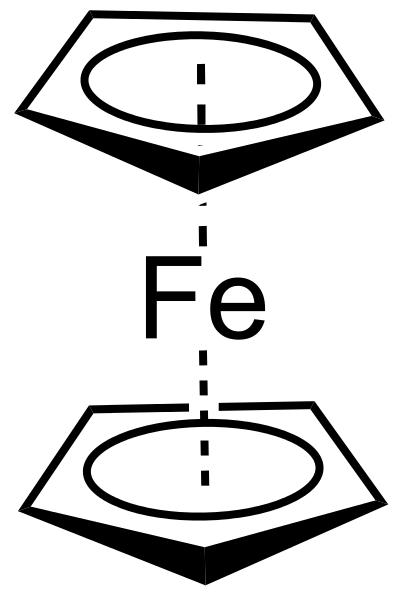
\includegraphics[width=0.1\linewidth]{ferrocene_structure.png}
    \caption{Strukturformel von Ferrocen.}
    \label{fig:ferrocen_struc}
\end{figure}

\subsubsection{Pulverartige Proben und magic angle}
Die oben genannten Intensitätsverteilungen der Peaks setzen voraus, dass in der untersuchten Probe keine Vorzugsrichtung besteht, so dass im Mittel die Winkelabhängigkeit der Abstrahlung verschwindet. \\
Für reine Quadrupolwechselwirkung und Zeemanaufspaltung existiert ein sogenannter \say{magic angle} von $\beta$, unter dem die Intensitätsverteilung genauso aussieht, als ob die Probe pulverartig wäre. Dieser Winkel beträgt etwa 54.7$^\circ$, weswegen dieser Wert im Fit pulverartiger Proben erwartet wird.


\section{Versuchsaufbau und benutzte Geräte}
\begin{enumerate}
    \item Kethley Spannungsmessgerät für $U_{Monitor}$
    \item Mößbauer Drive Unit (MBU)
    \item PC (Programm Moessfit)
    \item Function Generator
    \item MCA (Multi Channel Analysier) \& SCA (Single Channel Analyser)
\end{enumerate}

\section{Versuchsdurchführung}
Alle Teilexperimente wurden unter Zimmertemperatur durchgeführt. Die Rohdaten sind im Ordner \verb+C:\Fpraktikum\2021\22.10.21+ zu finden.
\subsection{Beschreibung der Signalverarbeitung}
Die Spannung an „CHA“, „START“, „Monitor" und „ANALOG Output“ wurde am Oszilloskop untersucht.\\
Der Channel-Anschluss sendet äquidistante quadratische Pulse alle 40 ms aus, er verbindet den Function Generator mit der CMCA. Der Start-Anschluss ist schwer zu beobachten, sendet aber auch quadratische Pulse aus, etwa alle 1000 CHA-Pulse. Er verbindet den Function Generator mit der Mössbauer Drive Unit. \\Das Monitor-Signal ist ein Sinus in der gleichen Frequenz wie das Start Signal, das so getaktet wird. Es wird auch an die Keithley-Messeinrichtung zum Ablesen der Maximalspannung weitergegeben. Der Analog Output gibt eine Sinus-Welle vom Function Generator zur MDU aus, womit die Geschwindigkeit gesteuert wird.
\subsection{Aufnahme von Pulshöhenspektren mit und ohne Probe}
Zunächst wird das gesamte Spektrum des $^{57}$Co-Strahlers im PHA-Modus aufgenommen (einmal mit, einmal ohne Probe), um den zu 14.4 keV gehörigen Peak mithilfe eines Vergleichsspektrums identifizieren zu können. 
\\In diesem Modus wird analog die durch einen Puls erzeugte Spannung analysiert und dann einem Channel (auf der x-Achse) zugeordnet. Die Zuordnung erfolgt linear. 
\\\\Die beiden Spektren sind in \bcref{fig:full_Spec} dargestellt, der für den Versuch relevante Peak ist gekennzeichnet. Die anderen Peaks rühren zum einen aus der Zerfallsreihe des Cobalt her, die auch einen Übergang mit 136 keV und einen mit 121.6 keV beinhaltet (dies sind die vorletzten beiden Peaks). Zum anderen entstehen sie als Konsequenz sekundärer Stöße der $\gamma$-Quanten mit den inneren Elektronen des Detektors und der Abschirmung, die diese Elektronen aus dem Atom lösen, woraufhin höher in der Hülle gelegene Elektronen sie ersetzen und dabei ein Photon abgegeben (analog zu einem charakteristischem Röntgenspektrum). Beispielhaft sei hier der Peak rechts der Compton-Kante (der maximal mögliche Energieübertrag durch Compton-Streuung) genannt, der der K$_{\alpha}$ Linie von Blei zuzuordnen ist. Des weiteren treten auch in der Bleihülle Resonanzabsorptionseffekte auf.
\\\\Die Skala ist logarithmisch, da die Peaks in höheren Channels sonst nicht erkennbar wären. Diese Darstellung verschleiert allerdings die Tatsache, dass die tatsächlich gemessenen Impulszahlen bei den hochenergetischen Channels zwischen der Messung mit und ohne Probe sehr viel näher beieinander liegen als bei den niederenergetischen Channels. \\\\Dieser abnehmende Unterschied ist darin begründet, dass die Probe die hochenergetische Strahlung rechts im Spektrum nicht mehr wirksam absorbieren kann, weshalb ihre Anwesenheit das Ergebnis weniger beeinflusst.\\%Weiß nicht ob das richtig ist
\begin{figure}[htp!]
    \centering
    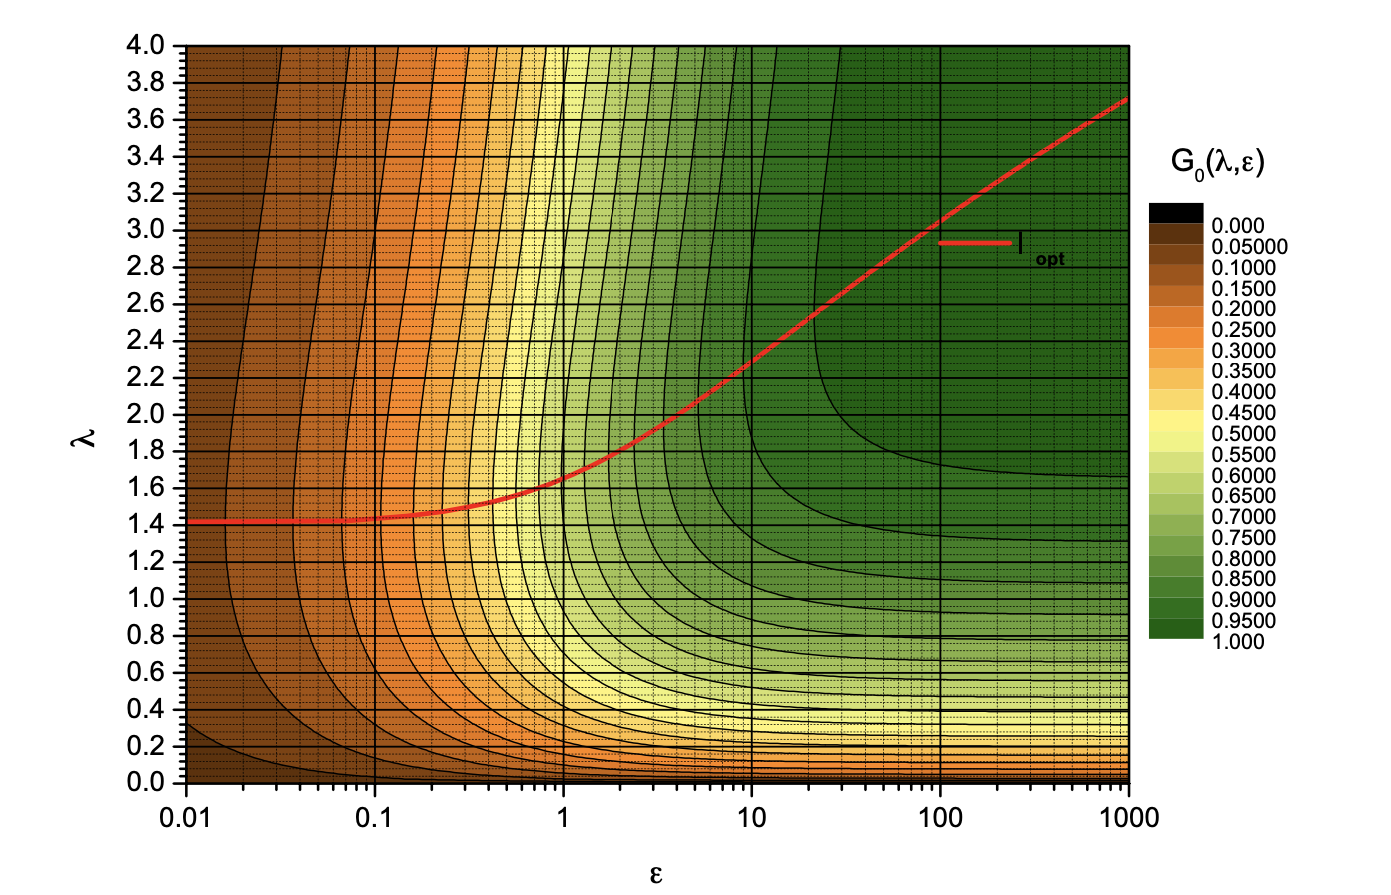
\includegraphics[width=0.55\linewidth]{mbs_guete.png}
    \caption{Güte $G_0$ des Mößbauerspektrums in Abhängigkeit der Breite $\lambda$ (Vielfache der Gaussbreite) des Gamma-Fensters und dem Verhältnis $\epsilon=\frac{S}{N}$ von Peakhöhe $S$ zu Untergrund $N$. Für ein gegebenes $\epsilon$ garantiert die Wahl von $\lambda_{opt}$ die kürzeste Messzeit.}
    \label{fig:guete}
\end{figure}
Nun wird die Breite des Peaks $\sigma$ auf 13.6 Channel abgeschätzt, das Zentrum wird bei Channel 28 verortet, und mittels \bcref{fig:guete} (aus der Versuchsanleitung) wird für $\epsilon=1.5$ ein $\lambda$ von etwa 1.7 bestimmt. $\lambda\cdot\sigma$ würde jetzt als Breite des beobachteten Bereichs um den Peak eingestellt werden, aber da die Ordinatenachse der Messung nicht richtig kalibriert war, mussten vom Betreuer gegebene Grenzen von $215\si{mV}-360\si{mV}$ verwendet werden. 
\begin{figure}[!htp]
    \centering
    \includesvg[width=0.8\linewidth]{spectra.svg}
    \caption{Pulshöhenspektrum mit und ohne Probe}
    \label{fig:full_Spec}
\end{figure}


\subsection{Kalibrierung des Mößbauerantriebs mit 25 \mum Eisen-Folie}
\label{kalibrierung}
Es folgt die Kalibrierung des Fits mittels einer $\SI{25}{\mu m}$ dicken $^{57}$Fe Folie, deren Mößbauerspektrum mit dem bekannten Hyperfeinfeld von 33.3 T verglichen wird, um den Parameter $\alpha$ für die Errechnung der Geschwindigkeit aus dem Channelsignal des Sinus-Wellengenerators zu bestimmen. Diese Messung findet bei einer Maximalspannung von 197.15 mV für etwa 30 min statt. Das aufgenommene Mößbauerspektrum ist in \bcref{fig:Mosskal} zu finden.\\
Mittels der Tatsache, dass die kalibrierte B-Feldstärke proportional zu der kalibrierten Maximalgeschwindigkeit des Dopplereffekts ist, und mit $\alpha:=\dfrac{v_\mathrm{max}}{U_\mathrm{Monitor}}$ findet man:
\begin{align}
    &\alpha_\mathrm{soll}=\alpha_\mathrm{test}\cdot\dfrac{B_\mathrm{soll}}{B_\mathrm{test}}
\end{align}
Der erste Fit mit $\alpha_\mathrm{test}=0.0646\si{\frac{mm}{smV}}$ ergab $B_\mathrm{test}=61.55$ T, somit wurde $\alpha_\mathrm{soll}=0.0349\si{\frac{mm}{smV}}$ ermittelt.\\
Im Programm \say{Moessfit} können Parameter vor dem Fit aus theoretischen Überlegungen festgesetzt werden. \\\\
Mit Fehlerfortpflanzung und den durch Moessfit gegebenen, als statistisch interpretierten Messunsicherheit des Parameters $B_{Test}$ ($\sigma_{B_{test}}=0.03\si{T}$)(die Messunsicherheiten von $B_{soll}$ und $\alpha_\mathrm{test}$ werden vereinfachend vernachlässigt) ergibt sich:
\begin{equation}
    \sigma_{\alpha_{soll}} = \alpha_{soll}\cdot  \left( \frac{\sigma_{B_{test}}}{B_{test}}\right) 
\end{equation}
Was einer relativen Messunsicherheit von $ \frac{ \sigma_{\alpha_{soll}}}{\alpha_{soll}}\approx 0.05\%$ entspricht.
\begin{figure}[h!]
    \centering
    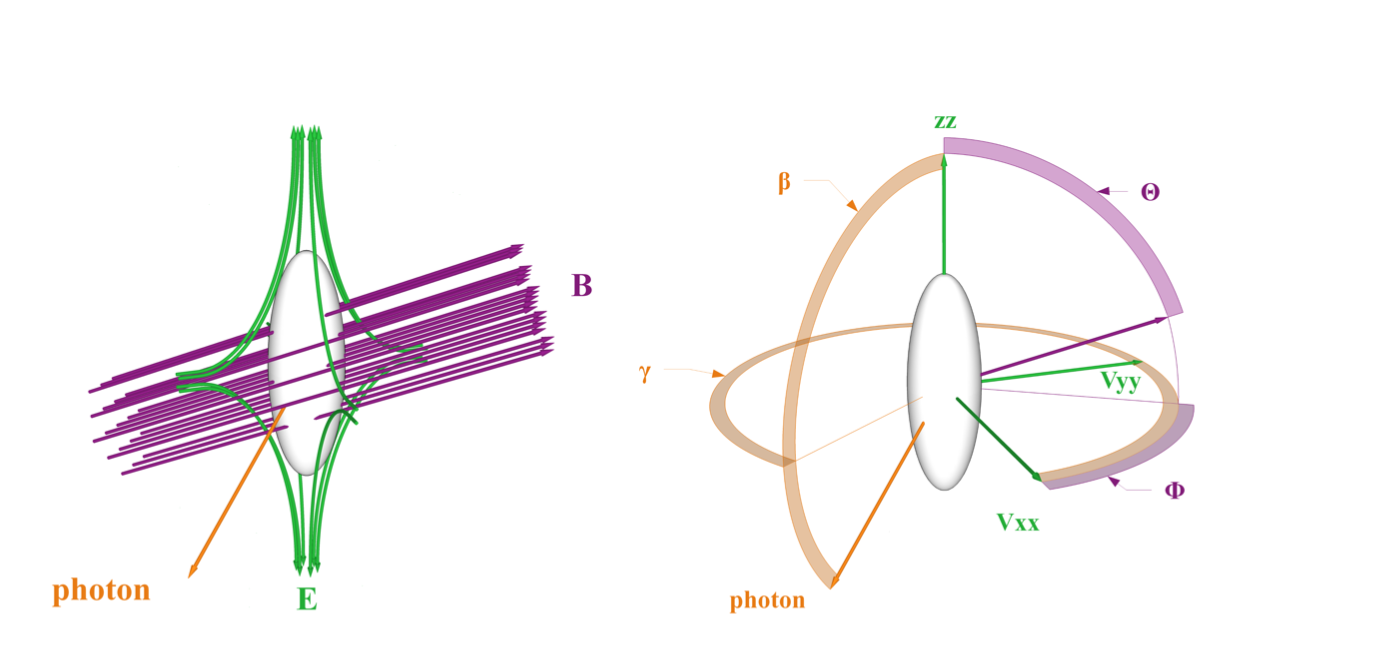
\includegraphics[width=0.9\linewidth]{mbs_parameter.png}
    \caption{Bedeutung der Texturwinkel $\beta$ und $\gamma$ sowie der Lage des magnetischen Hyperfeinfeldes beschrieben durch $\Theta$ und $\Phi$.}
    \label{fig:parameter}
\end{figure}\\
Im Fall von Eisenfolie wird aufgrund der sphärischen Ladungsverteilung kein Quadupolmoment und insbesondere keine Asymmetrie des Feldgradienten erwartet, weshalb die Parameter $V_{zz}, \eta, \theta, \varphi$ und $\gamma$ auf 0 gesetzt sind. Relevant ist auch, dass $\beta$, der Winkel zwischen Atomachse und eintreffender Strahlung, sehr nahe bei 54.7$^\circ$ liegt, dem magic angle, der eine pulverartige Probe beschreibt. 
\\Dies ist auch durch das erwartete 3:2:1:1:2:3 Verhältnis der Peaks erkenntlich. Dass er dennoch außerhalb der Messunsicherheit um diesen Punkt liegt, weißt auf ein gewisses Maß an Orientierung in der Probe hin, auf das in \bcref{3x4} näher eingegangen wird.\\
In der Tabelle bezeichnet $B_{Hyp}$ das Hyperfeinfeld des Atomkerns, CS den Centershift des Spektrums, $\omega$ die Linienbreite und $\beta$ den Polarwinkel zwischen eintreffendem Strahl und Materialausrichtung.\\ 
Der Fit gibt mit dem richtigen $\alpha_\mathrm{soll}$ die folgenden Parameter:
\begin{table}[!htp]
    \centering
    \begin{tabular}{c|c}
    Parameter&Wert\\\hline
        $B_{Hyp}$&(33.25$\pm$0.02) T \\
        CS&(-0.1082$\pm$0.0021)\si{\frac{mm}{s}}\\
        $\omega$&(0.1935$\pm$0.0034)\si{\frac{mm}{s}}\\
        $\beta$&(56.8$\pm$0.5)$^\circ$
    \end{tabular}
    \caption{Fitparameter der (richtig kalibrierten) Kalibrierungsmessung.}
    \label{tab:my_label}
\end{table}
\begin{figure}[!htp]
    \centering
    \includesvg[width=\linewidth]{3Fe25197.svg}
    \caption{Kalibrierung mittels 25\mum Eisenfolie.}
    \label{fig:Mosskal}
\end{figure}
\pagebreak

\subsection{$\protect 3 \times4\mum\:^{57}$Fe Folie}\label{3x4}
Jetzt wird die selbe Messung mit 4 jeweils 3 \mum dicken hintereinander angeordneten $^{57}$Fe Folien wiederholt. Das dort aufgenommene Spektrum ist in \bcref{fig:4x3} zu finden. $a$ in \bcref{tab:4x3} beschreibt den Anteil von unausgerichteten Domänen in der Folie.
\begin{table}[!htp]
    \centering
    \begin{tabular}{c|c}
    Parameter&Wert\\\hline
        $B_{Hyp}$&(33.28$\pm$0.02) T \\
        CS&(-0.1086$\pm$0.0022)\si{\frac{mm}{s}}\\ 
        $\omega$&(0.1603$\pm$0.0033)\si{\frac{mm}{s}}\\
        $\beta$&(63.8$\pm$0.7)$^\circ$\\
        $a$&0.583$\pm$0.028
    \end{tabular}
    \caption{Fitparameter der dünnen Folien. Es gelten die selben Argumente für das verschwinden gewisser Parameter wie in \bcref{kalibrierung}.}
    \label{tab:4x3}
\end{table}
\paragraph{Zum $\beta$ Winkel}Die Abweichung von $\beta$ von 54.7$^\circ$ ist beträchtlich stärker als noch bei der 25 \mum Folie, was auf eine recht deutliche Strukturierung der Probe hinweist. Der abweichende Winkel wird auch dadurch erkennbar, dass der zweite und fünfte Peak weit größer sind als von einer pulverförmigen Probe erwartet würde. \\\\Die Hypothese wurde aufgestellt, dass sich innerhalb von magnetischen Domänen an den Außenseiten der Folien die Spins zur Energieminimierung parallel zur Oberfläche ausrichten, was zu einem $\beta$ von 90$^\circ$ in diesen Bereichen führt. Innerhalb der Folie sind die Domänen aber weiterhin pulverartig verteilt, was erklärt, warum der Effekt bei der dickeren 25\mum Folie weit weniger drastisch ausfällt (da dort ein weit geringeres Verhältnis von Oberfläche zu Volumen vorhanden ist). \\Um diesen Effekt zu quantifizieren, wurde der Parameter $a$ eingeführt. Das Fitmodell wurde dann umgeschrieben zu einer Addition von unausgerichteten und ausgerichteten Anteil, die in \bcref{fig:4x3} gut zu erkennen sind. \\\\
Mithilfe von $a$ und der bekannten Dicke der Folie lassen sich nun Rückschlüsse über die Größe von magnetischen Domänen in Eisen erlauben. Unter der Annahme, dass die Domänen (eine auf der Vorderseite, eine auf der Rückseite) die gesamte Fläche ausfüllen (da die anderen Randgebiete klein sind), kann man schließen, dass:
\begin{align}
    &d_\text{Domäne}=\frac{d_\mathrm{Folie}\cdot(1-a)}{2}=0.83\mum
\end{align}
Der Fehler wird nur durch die Unsicherheit von $a$ bedingt und beträgt deshalb $0.039\mum$ (4.8\% der Größe, wie $a$).
\begin{figure}[!htp]
    \centering
    \includesvg[width=\linewidth]{2Fe4x3197mod.svg}
    \caption{Mößbauerspektrum der drei Eisenfolien, aufgespaltet nach magnetischen Domänen.}
    \label{fig:4x3}
\end{figure}


\subsection{Ferrocen}
Als nächstes sollte Ferrocen bei deutlich niedrigerer Maximalspannung (etwa 115 mV) gemessen werden, allerdings machten technische Probleme mit dem Versuchsaufbau die Aufnahme eines brauchbaren Spektrums unmöglich, weswegen Messergebnisse aus dem letzten F-Praktikum benutzt wurden. Diese sind in \bcref{fig:Ferrocen}  dargestellt. In \bcref{tab:ferrocen} beschreibt $V_{zz}$ die $zz$ Komponente des Feldgradienten und $\theta$ und $\varphi$ die Winkel zwischen magnetischem Feld und elektrischem Feldgradienten.\\
\label{ferrocen}
\begin{table}[!htp]
    \centering
    \begin{tabular}{c|c}
    Parameter&Wert\\\hline
        $B_{Hyp}$&(0$\pm$0.02) T \\
        $V_{zz}$&(141.7$\pm$0.5) $\si{\frac{V}{\angstrom^2}}$ \\
        $\theta$&$-20.7^\circ$\\
        $\varphi$&$-73.6^\circ$\\
        CS&(0.328$\pm$0.004)\si{\frac{mm}{s}}\\ 
        $\omega$&(0.121$\pm$0.006)\si{\frac{mm}{s}}\\
        $\beta$&(52.3$\pm$2.0)$^\circ$
    \end{tabular}
    \caption{Fitparameter von Ferrocen.}
    \label{tab:ferrocen}
\end{table}
\begin{figure}[!h]
    \centering
    \includesvg[width=\linewidth]{5Ferrocen.svg}
    \caption{Mößbauerspektrum des Ferrocen mit gut erkennbarer Quadrupolaufspaltung (Dublett)}
    \label{fig:Ferrocen}
\end{figure}\\
Der Isomerieshift $\Delta$, bezogen auf den im Eisensextett kann berechnet werden als:
\begin{align}
    \Delta=CS_\text{Ferrocen}-CS_\text{ 25 $\mu$m Fe-Folie}=(0.328+0.1082)\si{\frac{mm}{s}}=0.4362\si{\frac{mm}{s}}.
\end{align}

Man beobachtet eine charakteristische Dublett-Quadrupolaufspaltung, aufgrund der nicht kugelsymmetrischen Ladungsverteilung außerhalb des Eisenatoms, wobei die beiden sichtbaren Peaks jeweils zu den jeweils zweifach entarteten Zuständen $I_z=1/2, \,\,3/2$ zu $I=3/2$ gehören. Das resultiert in einem relativ großen $V_{zz}$-Faktor.\\\\
Der Parameter $\beta$ liegt innerhalb der Fehlergrenze bei dem magic angle ($\approx 54,7^{\circ}$), was auf eine pulverartige Struktur der (sandwichartig) eingebetteten Eisenkerne in die (\ce{C5H5})-Gruppen schließen lässt. Dennoch ist in \bcref{fig:Ferrocen} deutlich die Asymetrie der Peaks zu erkennen. \\\\Diese Asymetrie könnte hauptsächlich durch den Goldanskii-Karyagin Effekt oder durch einen Textureffekt (beispielsweise durch eine bevorzugte Liegerichtung der Ferrocen-Moleküle) erklärt werden. Dies würde untersucht, indem die Probe rotiert wird. Die spezielle Änderung der Asymetrie lässt eine Entscheidung über die wahrscheinliche Ursache zu.\footnote{vgl. U. Gonser, H.-D. Pfannes. TEXTURE PROBLEMS. Journal de Physique Colloques, 1974, 35 (C6),
pp.C6-113-C6-120. 10.1051/jphyscol:1974610 . jpa-00215710} Diese Messung wurde nicht durchgeführt, Herr Seewald hatte aber den Goldanskii-Karyagin Effekt als Ursache ausgeschlossen. Entsprechend ist ein Textureffekt die bevorzugte Erklärung.\\\\
Umso interessanter ist, dass in dem Spektrum keine Kern-Zeeman-Aufspaltung erkennbar ist, die man aufgrund der pulverhaftigkeit, bzw. der ferromagnetischen Natur der $^{57}$Fe-Atomen erwarten würde. Die Aufspaltung würde durch ein Magnetfeld zustande kommen (Vgl. \bcref{zeeman}), wobei in diesem Fall kein äußeres vorliegt, sondern, wenn überhaupt eines aufgrund der lokalen magnetischen Momente ungepaarter Elektronen erzeugt würde. \\
Dies lässt nur den Rückschluss zu, dass in der Bindungskonfiguration des Fe-Atoms mit den Kohlenwasserstoffgruppen keine ungepaarten Elektronen vorliegen, was in dem Fitparameter in \bcref{tab:ferrocen} resultiert.\footnote{Vgl. Didzoleit, H., 2016, Struktur und Magnetismus von Ferrocen und ferrocenhaltigen Polymeren in dünnen Filmen, S. 123, \href{https://tuprints.ulb.tu-darmstadt.de/5317/1/thesis_finalVersion.pdf}{\textcolor{blue}{Link}}}
Der Center-Shift ist auf die Isomerieverschiebung des $14,4$ keV-Niveau der $^{57}$Fe-Kerne im Ferrocen ggü. den $^{57}$Fe-Kernen, die aus der Zerfallsreihe des $^{57}$Co zurückzuführen.
\paragraph{Feldberechnung}
Da in Ferrocen offensichtlich nur die Quadrupol- Hyperfeinwechselwirkung eine Rolle spielt und diese aufgrund elektromagnetischer Wechselwirkungen herrührt, bietet es sich hier an mit einfachen Mitteln der Elektrodynamik in Näherung das elektrostatische Potential $\Phi$ von Ferrocen zu berechnen, indem man die positive Ladung im gewählten Koordinatenmittelpunkt vernachlässigt und die beiden Kohlenwasserstoffgruppen als gleichverteilte Felddichten von Punktladungen betrachtet, was sinnvoll ist, da aufgrund der Symmetrie der Gruppe, die Elektronen delokalisiert sind und sich uniform in den Ringen verteilen.\\\\
Mit $\Phi$ soll dann in Abhängigkeit des Abstands $d$ vom Koordinatenmittelpunkt (Eisenatom) die $V_{zz}$-Komponente des elektrischen  Feldgradienten $V_{ij}$ berechnet werden (ein symmetrischer Tensor 2. Stufe mit verschwindender Spur).\\\\
Man macht sich hier die Geometrie zu nutze und begibt sich in das Hauptachsensystem des Feldgradienten, wobei die $z$-Achse mit der Verbindungsachse der beiden Kohlenwasserstoffgruppen übereinstimmt, welche orthogonal auf diesen steht und durch das Eisenkation verläuft. \\\\
Auf Grund der Radialsymmetrie um diese Achse ist klar, dass $V_{xx} = V_{yy}$ und $V_{ij}=0 \,\,\, \forall i \ne j $, wobei der elektrische Feldgradient hier ohnehin Diagonalgestalt hat, was in dem Asymmetrieparameter $\eta := \frac{V_{xx}-V_{yy}}{V_{zz}} = 0$ resultiert.\\\\
Man nutzt im Weiteren die bereits in \bcref{quad} eingeführte Beschreibung des elektrischen Feldgradienten.\\
Mit den Annahmen über die Ladungsverteilung hat das elektrostatische Potential diese Gestalt, wobei man sich nun auf die $z$-Achse beschränkt und den Nullpunkt, wie gesagt in die Position des Fe-Atoms legt:
\begin{equation}
    \Phi(z) = \frac{e}{4 \pi \epsilon_0}\left (\frac{1}{|z-d|} + \frac{1}{|z+d|} \right)
\end{equation}
Es ergibt sich:
\begin{align}
    \frac{\partial \Phi(z)}{\partial z} = & -\frac{e}{4 \pi \epsilon_0}\left (\frac{1}{(z-d)|z-d|} + \frac{1}{(z+d)|z+d|} \right)\\
    \frac{\partial^2 \Phi(z)}{\partial z^2} =& \frac{e}{2 \pi \epsilon_0}\left (\frac{1}{(z-d)^2|z-d|} + \frac{1}{(z+d)^2|z+d|} \right)
\end{align}
Und somit für die Komponente des elektrischen Feldgradienten im Koordinatenmittelpunkt:
\begin{equation}
    V_{zz}(z=0) = \Phi_{zz} = \frac{e}{2 \pi \epsilon_0}\left (\frac{1}{d^3}+\frac{1}{d^3} \right) = \frac{e}{\pi \epsilon_0\cdot d^3}
\end{equation}
Daraus folgt mit dem Wert aus \bcref{tab:ferrocen} für $V_{zz}$, dass
\begin{align}
    d = \sqrt[3]{\dfrac{e}{\pi\epsilon_0V_{zz}}}=0.74\si{\angstrom}. 
\end{align}
Dies entspricht 45\% des Abstandes der Cyclopentadienylringe vom zentralen Eisen-Atom (Literaturwert: $d_{lit.}=1,66 \si{\angstrom}$).\footnote{Vgl. https://de.wikipedia.org/wiki/Ferrocen, Stand: 31.10.2021}

\subsection{Unbekannte Probe}
\label{mystery}
Als Zusatzaufgabe wird das Spektrum einer unbekannten Probe, wieder bei 286 mV,
allerdings 55 Minuten lang, aufgenommen, das in \bcref{fig:mystery} dargestellt ist.
\begin{table}[!htp]
    \centering
    \begin{tabular}{c|c}
    Parameter&Wert\\\hline
        $B_{Hyp}$&(51.53$\pm$0.03) T \\
        $V_{zz}$&(-7.37$\pm$0.5) $\si{\frac{V}{\angstrom^2}}$ \\
        CS&(0.248$\pm$0.004)\si{\frac{mm}{s}}\\ 
        $\omega$&(0.284$\pm$0.006)\si{\frac{mm}{s}}\\
        $\beta$&(57.2$\pm$0.6)$^\circ$\\
    \end{tabular} 
    \caption{Fitparameter der unbekannten Probe.}
    \label{tab:mystery}
\end{table}
\begin{figure}[!h]
    \centering
    \includesvg[width=\linewidth]{4mystery.svg}
    \caption{Spektrum der unbekannten Probe.}
    \label{fig:mystery}
\end{figure}
Auffällig ist hier, neben den unten genannten Parametern, dass das Fitmodell die inneren beiden Peaks nicht angemessen skalieren kann. Dies könnte dadurch erklärt werden, dass das Modell eines einfachen Kristalls nicht angemessen ist.\\
Es wurde vom Betreuer mitgeteilt, dass die Struktur der Probe aus den Atomen Fe, C und O besteht, und die Kristallstrukturen $\ce{Fe3O4}$, $\ce{Fe2O5}$ und $\ce{FeC2}$ ausgeschlossen werden können.\\\\
Die Messung an der Probe zeigt deutlich die Sextett-Struktur der Kern-Zeemanaufspaltung, was auf ein nicht verschwindendes $B_{Hyp}$ rückschließen lässt (wie bei den vorher betrachteten Eisenfolien verschiedener Dicke).\\
Der Texturwinkel $\beta=57.2^{\circ}$, der sehr nah am magic angle ist deutet auf eine pulverartige Struktur hin (was durch die Linienintensitätsverhältnisse 3:2:1:1:2:3 noch deutlicher wird).\\\\
Recherche nach gängigen Eisenoxiden bzw. Eisenkarbiden führt zu dem gesuchten Kandidaten: Hämatit.\\
%\href{https://link.springer.com/content/pdf/10.1007/BF00307402.pdf}{\textcolor{blue}{Dieses}} Paper\footnote{C.A.  Mc Cammon and D.C. Price, Mössbauer Spectra of $Fe_xO$ ($x>0.95$), Phys Chem Minerals (1985) 11:250-254} schließt $\ce{FeO}$ aufgrund der ungleichen Peakstruktur im Vergleich zu \bcref{fig:mystery} und des Isomerieshifts von $\delta \approx 1$ im Vergleich zu \bcref{tab:mystery} aus. Mit Argumenten des chemischen Aufbaus wird $\ce{Fe2O}$ deshalb auch ausgeschlossen.\\
%\href{https://pubs.rsc.org/en/content/articlepdf/2014/ra/c4ra11283k}{\textcolor{blue}{Folgende}} Arbeit\footnote{Srividhya J. Iyengar, Mathew Joy, Chandan Kumar Ghosh, Subhrajyoti Dey, Ravinder K. Kotnalad and Swapankumar Ghosh, Magnetic, X-ray and Mössbauer studies on magnetite/maghemite core–shell nanostructures fabricated through an aqueous route, RSC Advances 110, 2014} schließt das sogenannte Magnetit, $\ce{Fe2O3}$ aus. Die Spektren sich auch hier wieder sehr unähnlich sind, bzgl. der Lage der Peaks und der Symmetrie des Spektrums
%Das Spektrum weißt zwar ein charakteristisches Sextett auf, allerdings stimmen die Linienverhältnisse nicht mit der Mystery Probe überein.\\\\
 \href{http://dx.doi.org/10.4028/www.scientific.net/JMNM.20-21.641}{\textcolor{blue}{Dieses}} Paper\footnote{Mashlan M. et al., 2004, Mössbauer Spectroscopy in Study of Thermally Induced Crystallization of Amorphous $\alpha-\ce{Fe2O3}$ Nanoparticles} bestätigt das. Das Spektrum des $\alpha-\ce{Fe2O3}$ weißt das charakteristische Zeeman-Sextett auf, außerdem stimmen hier nun auch die Linienintensitätsverhältnisse mit der Mystery-Probe überein. Dazu kommt, dass die Minima das Sextetts zufriedenstellend genau mit denen aus \bcref{fig:mystery} übereinstimmen.\\
 Ein Vergleich der Parameter bringt Gewissheit: \\$B^{lit.}_{Hyp} = 51.7 \si{T}$ (Bei $300 \si{K}$) vs. $B_{hyp} = 51.53 \si{T}$ und den Isomerieshifts\\ $\Delta_\text{Mystery} = CS_\text{Mystery} - CS_\text{ 25 $\mu$m Fe-Folie} = 0.356 \si{\frac{mm}{s}}$ vs. $\Delta_{lit.} = 0.37 \si{\frac{mm}{s}}$ \\
 mit den Werten aus \bcref{tab:mystery}.
\newpage
\section{Diskussion}
Die Spektren haben die erwartete Form mit reinem Sextett/Dublett.\\
In \say{Physics of Ferromagnetism} wird zur Berechnung für der Domänendicke von Eisen 
\begin{align}
&d=3.04\ten{-3}\frac{\sqrt{1.6\ten{-3}\cdot l}}{2.15}
\end{align}
angegeben\footnote{Chikazumi, S., Physics of Ferromagnetism (1997), 2nd ed., S.  441. Oxford: Clarendon Press.}, wobei $l$ die Dicke der Folie beschreibt.  In unserem Fall ergäbe dies eine Domänendicke von 0.12\mum, innerhalb der Messunsicherheit ein Siebtel der 0.83\mum aus unserer Abschätzung. Dies ist nicht sonderlich überraschend, da die parallel zur Oberfläche ausgerichtete Schicht durchaus mehrere Domänen umfassen kann, die um 180$^\circ$ gegeneinander rotiert sind.\\\\
Für Ferrocen lässt sich
der Isomerieshift von 0.4362 \si{\frac{mm}{s}} durch Vergleich mit einschlägigen Tabellen bestimmen, da der Oxidationszustand mit +II bekannt ist. Man findet, dass der Spinzustand entweder $S=0$ oder $S=1$ ist, da dieser Isomerieshift von beiden Zuständen erreicht werden kann.\\\\
Unser Ergebnis für den Abstand des Eisens von dem Kohlenwasserstoffring von 0.74 \si{\angstrom} sind etwa 45\% des tatsächlichen Abstandes von 3.32/2 \si{\angstrom} .\footnote{https://de.wikipedia.org/wiki/Ferrocen, Stand: 31.10.2021} In Anbetracht der zahlreichen Vereinfachungen (Punktladungen, Vernachlässigung der Positiven Ladung des Eisen, negative Ladung genau am Kohlenwasserstoffring anstatt zwischen Eisen und Kohlenwasserstoff) ist dies ein zu erwartendes Ergebnis.\\\\
Die unbekannte Probe konnte zu Hämatit ($\alpha-\ce{Fe2O3}$) bestimmt werden, wobei die Hyperfeinparameter sehr gut mit denen einer anderen (Vgl. \bcref{mystery}) Messung übereinstimmen.\\\\
Ein Verbesserungsvorschlag für eine genauere Messung und damit genaueren Hyperfeinparametern wäre die Messung unter niedrigen Temperaturen, da somit Gitterschwingungen des Absorbermaterials reduziert werden können, was zu einer genaueren Auflösung der Transmissionsspektren (insbesondere der Minima) führt.

%\section{Appendix}
%\label{appendix}
%\printbibliography
%\begin{itemize}
 %   \item %unser Slub Buch
    
  %  \item % Praktikumsskript
%\end{itemize}

\end{document}